% Z_2 as a binary tree (generated; see Chapter 12).
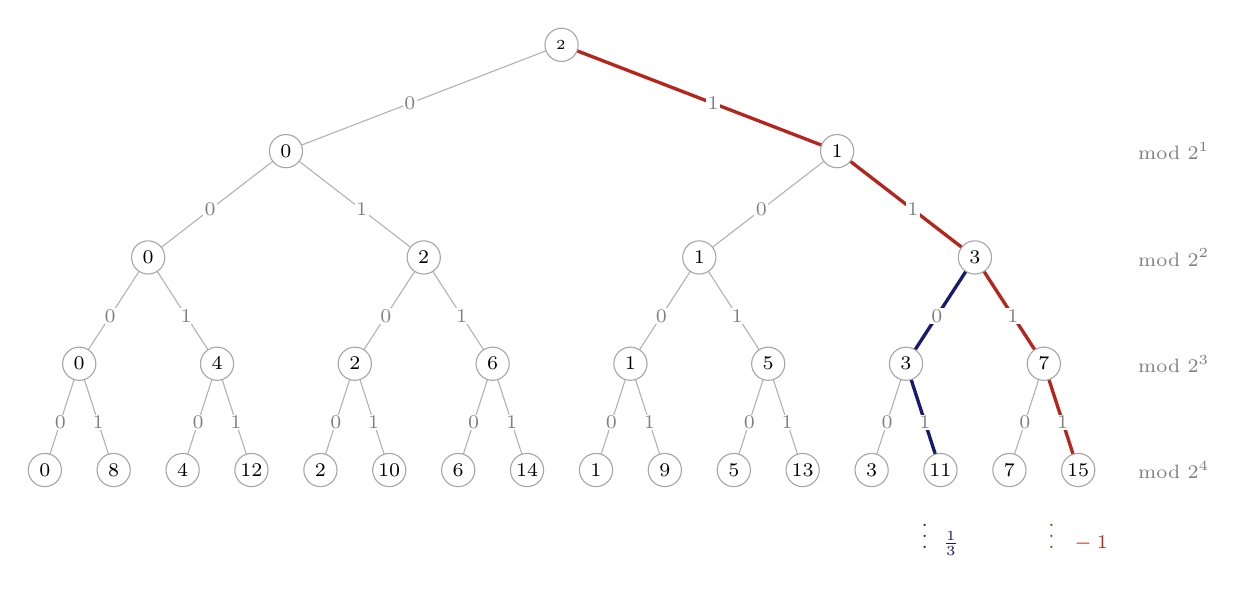
\begin{tikzpicture}[font=\scriptsize]
  \draw[gray!60,thin] (7.000,0.000) -- node[pos=0.55,fill=white,inner sep=0.5pt,text=gray] {0} (3.500,-1.350);
  \draw[BrickRed,very thick] (7.000,0.000) -- node[pos=0.55,fill=white,inner sep=0.5pt,text=gray] {1} (10.500,-1.350);
  \draw[gray!60,thin] (3.500,-1.350) -- node[pos=0.55,fill=white,inner sep=0.5pt,text=gray] {0} (1.750,-2.700);
  \draw[gray!60,thin] (3.500,-1.350) -- node[pos=0.55,fill=white,inner sep=0.5pt,text=gray] {1} (5.250,-2.700);
  \draw[gray!60,thin] (10.500,-1.350) -- node[pos=0.55,fill=white,inner sep=0.5pt,text=gray] {0} (8.750,-2.700);
  \draw[BrickRed,very thick] (10.500,-1.350) -- node[pos=0.55,fill=white,inner sep=0.5pt,text=gray] {1} (12.250,-2.700);
  \draw[gray!60,thin] (1.750,-2.700) -- node[pos=0.55,fill=white,inner sep=0.5pt,text=gray] {0} (0.875,-4.050);
  \draw[gray!60,thin] (1.750,-2.700) -- node[pos=0.55,fill=white,inner sep=0.5pt,text=gray] {1} (2.625,-4.050);
  \draw[gray!60,thin] (5.250,-2.700) -- node[pos=0.55,fill=white,inner sep=0.5pt,text=gray] {0} (4.375,-4.050);
  \draw[gray!60,thin] (5.250,-2.700) -- node[pos=0.55,fill=white,inner sep=0.5pt,text=gray] {1} (6.125,-4.050);
  \draw[gray!60,thin] (8.750,-2.700) -- node[pos=0.55,fill=white,inner sep=0.5pt,text=gray] {0} (7.875,-4.050);
  \draw[gray!60,thin] (8.750,-2.700) -- node[pos=0.55,fill=white,inner sep=0.5pt,text=gray] {1} (9.625,-4.050);
  \draw[MidnightBlue,very thick] (12.250,-2.700) -- node[pos=0.55,fill=white,inner sep=0.5pt,text=gray] {0} (11.375,-4.050);
  \draw[BrickRed,very thick] (12.250,-2.700) -- node[pos=0.55,fill=white,inner sep=0.5pt,text=gray] {1} (13.125,-4.050);
  \draw[gray!60,thin] (0.875,-4.050) -- node[pos=0.55,fill=white,inner sep=0.5pt,text=gray] {0} (0.438,-5.400);
  \draw[gray!60,thin] (0.875,-4.050) -- node[pos=0.55,fill=white,inner sep=0.5pt,text=gray] {1} (1.312,-5.400);
  \draw[gray!60,thin] (2.625,-4.050) -- node[pos=0.55,fill=white,inner sep=0.5pt,text=gray] {0} (2.188,-5.400);
  \draw[gray!60,thin] (2.625,-4.050) -- node[pos=0.55,fill=white,inner sep=0.5pt,text=gray] {1} (3.062,-5.400);
  \draw[gray!60,thin] (4.375,-4.050) -- node[pos=0.55,fill=white,inner sep=0.5pt,text=gray] {0} (3.938,-5.400);
  \draw[gray!60,thin] (4.375,-4.050) -- node[pos=0.55,fill=white,inner sep=0.5pt,text=gray] {1} (4.812,-5.400);
  \draw[gray!60,thin] (6.125,-4.050) -- node[pos=0.55,fill=white,inner sep=0.5pt,text=gray] {0} (5.688,-5.400);
  \draw[gray!60,thin] (6.125,-4.050) -- node[pos=0.55,fill=white,inner sep=0.5pt,text=gray] {1} (6.562,-5.400);
  \draw[gray!60,thin] (7.875,-4.050) -- node[pos=0.55,fill=white,inner sep=0.5pt,text=gray] {0} (7.438,-5.400);
  \draw[gray!60,thin] (7.875,-4.050) -- node[pos=0.55,fill=white,inner sep=0.5pt,text=gray] {1} (8.312,-5.400);
  \draw[gray!60,thin] (9.625,-4.050) -- node[pos=0.55,fill=white,inner sep=0.5pt,text=gray] {0} (9.188,-5.400);
  \draw[gray!60,thin] (9.625,-4.050) -- node[pos=0.55,fill=white,inner sep=0.5pt,text=gray] {1} (10.062,-5.400);
  \draw[gray!60,thin] (11.375,-4.050) -- node[pos=0.55,fill=white,inner sep=0.5pt,text=gray] {0} (10.938,-5.400);
  \draw[MidnightBlue,very thick] (11.375,-4.050) -- node[pos=0.55,fill=white,inner sep=0.5pt,text=gray] {1} (11.812,-5.400);
  \draw[gray!60,thin] (13.125,-4.050) -- node[pos=0.55,fill=white,inner sep=0.5pt,text=gray] {0} (12.688,-5.400);
  \draw[BrickRed,very thick] (13.125,-4.050) -- node[pos=0.55,fill=white,inner sep=0.5pt,text=gray] {1} (13.562,-5.400);
  \node[circle,fill=white,draw=gray!70,inner sep=1pt,minimum size=12pt] at (7.000,0.000) {$\Z_2$};
  \node[circle,fill=white,draw=gray!70,inner sep=1pt,minimum size=12pt] at (3.500,-1.350) {$0$};
  \node[circle,fill=white,draw=gray!70,inner sep=1pt,minimum size=12pt] at (10.500,-1.350) {$1$};
  \node[circle,fill=white,draw=gray!70,inner sep=1pt,minimum size=12pt] at (1.750,-2.700) {$0$};
  \node[circle,fill=white,draw=gray!70,inner sep=1pt,minimum size=12pt] at (5.250,-2.700) {$2$};
  \node[circle,fill=white,draw=gray!70,inner sep=1pt,minimum size=12pt] at (8.750,-2.700) {$1$};
  \node[circle,fill=white,draw=gray!70,inner sep=1pt,minimum size=12pt] at (12.250,-2.700) {$3$};
  \node[circle,fill=white,draw=gray!70,inner sep=1pt,minimum size=12pt] at (0.875,-4.050) {$0$};
  \node[circle,fill=white,draw=gray!70,inner sep=1pt,minimum size=12pt] at (2.625,-4.050) {$4$};
  \node[circle,fill=white,draw=gray!70,inner sep=1pt,minimum size=12pt] at (4.375,-4.050) {$2$};
  \node[circle,fill=white,draw=gray!70,inner sep=1pt,minimum size=12pt] at (6.125,-4.050) {$6$};
  \node[circle,fill=white,draw=gray!70,inner sep=1pt,minimum size=12pt] at (7.875,-4.050) {$1$};
  \node[circle,fill=white,draw=gray!70,inner sep=1pt,minimum size=12pt] at (9.625,-4.050) {$5$};
  \node[circle,fill=white,draw=gray!70,inner sep=1pt,minimum size=12pt] at (11.375,-4.050) {$3$};
  \node[circle,fill=white,draw=gray!70,inner sep=1pt,minimum size=12pt] at (13.125,-4.050) {$7$};
  \node[circle,fill=white,draw=gray!70,inner sep=1pt,minimum size=12pt] at (0.438,-5.400) {0};
  \node[circle,fill=white,draw=gray!70,inner sep=1pt,minimum size=12pt] at (1.312,-5.400) {8};
  \node[circle,fill=white,draw=gray!70,inner sep=1pt,minimum size=12pt] at (2.188,-5.400) {4};
  \node[circle,fill=white,draw=gray!70,inner sep=1pt,minimum size=12pt] at (3.062,-5.400) {12};
  \node[circle,fill=white,draw=gray!70,inner sep=1pt,minimum size=12pt] at (3.938,-5.400) {2};
  \node[circle,fill=white,draw=gray!70,inner sep=1pt,minimum size=12pt] at (4.812,-5.400) {10};
  \node[circle,fill=white,draw=gray!70,inner sep=1pt,minimum size=12pt] at (5.688,-5.400) {6};
  \node[circle,fill=white,draw=gray!70,inner sep=1pt,minimum size=12pt] at (6.562,-5.400) {14};
  \node[circle,fill=white,draw=gray!70,inner sep=1pt,minimum size=12pt] at (7.438,-5.400) {1};
  \node[circle,fill=white,draw=gray!70,inner sep=1pt,minimum size=12pt] at (8.312,-5.400) {9};
  \node[circle,fill=white,draw=gray!70,inner sep=1pt,minimum size=12pt] at (9.188,-5.400) {5};
  \node[circle,fill=white,draw=gray!70,inner sep=1pt,minimum size=12pt] at (10.062,-5.400) {13};
  \node[circle,fill=white,draw=gray!70,inner sep=1pt,minimum size=12pt] at (10.938,-5.400) {3};
  \node[circle,fill=white,draw=gray!70,inner sep=1pt,minimum size=12pt] at (11.812,-5.400) {11};
  \node[circle,fill=white,draw=gray!70,inner sep=1pt,minimum size=12pt] at (12.688,-5.400) {7};
  \node[circle,fill=white,draw=gray!70,inner sep=1pt,minimum size=12pt] at (13.562,-5.400) {15};
  \node[anchor=west,text=gray] at (14.20,-1.35) {mod $2^{1}$};
  \node[anchor=west,text=gray] at (14.20,-2.70) {mod $2^{2}$};
  \node[anchor=west,text=gray] at (14.20,-4.05) {mod $2^{3}$};
  \node[anchor=west,text=gray] at (14.20,-5.40) {mod $2^{4}$};
  \node[anchor=north,BrickRed] at (13.56,-5.75) {$\vdots\ \ -1$};
  \node[anchor=north,MidnightBlue] at (11.81,-5.75) {$\vdots\ \ \frac13$};
\end{tikzpicture}
